%        File: HW.tex
%     Created: 二 6月 12 12:00 上午 2018 C
% Last Change: 二 6月 12 12:00 上午 2018 C
%
\documentclass[UTF8,noindent]{ctexart}
\usepackage[a4paper,left=2.0cm,right=2.0cm,top=2.0cm,bottom=2.0cm]{geometry}
\usepackage{hyperref}
\usepackage{arydshln}
\usepackage{url}
\usepackage{graphicx}
\usepackage{amsmath}
\usepackage{amssymb}
\usepackage{enumitem}
\usepackage{tikz}
\usepackage{forest}
\usepackage{float}
\usepackage{listings}
\usepackage{xcolor}
\lstset{language = c,numbers=left, keywordstyle= \color{ blue!70 },commentstyle=\color{red!50!green!50!blue!50}, frame=shadowbox, rulesepcolor= \color{ red!20!green!20!blue!20 } 
} 
\usetikzlibrary{graphs}
\title{$Chapter\ 7-HW$}
\author{$2015K8009929049$\ 冯吕}
\date{\today}

\begin{document}
\maketitle
\zihao{5}
\CJKfamily{zhsong}
$7.2.4$解:栈的活动记录如下图所示:
%\begin{center}
%  \begin{tabular}{|c|}
%    \hline
%    \\
%    \hline
%    $int\ y$\\
%    \hdashline
%    $g(y)$\\
%    \hdashline
%    $point \ to \ caller\ of \ g$\\
%    \hdashline
%    $int\ j$\\
%    \hline
%    $int\ x$\\
%    \hdashline
%    $f(x)$\\
%    \hdashline
%    $point\ to\ g$\\
%    \hdashline
%    $int \ i$\\
%    \hline
%  \end{tabular}
%\end{center}
\begin{figure}[H]
  \centering
  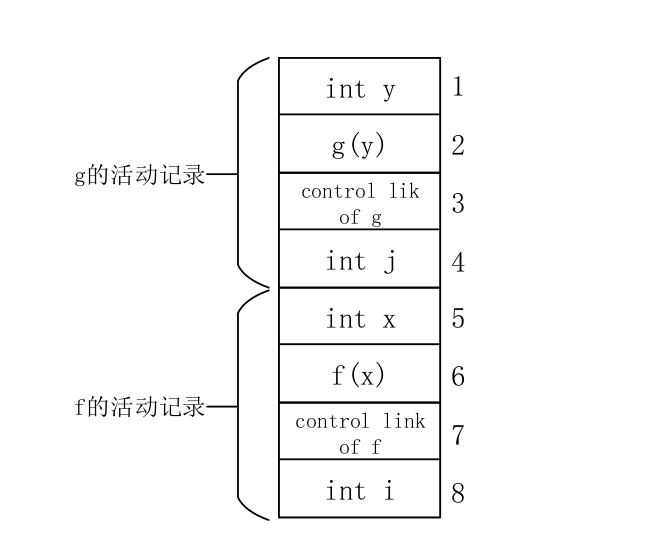
\includegraphics[scale = 0.4]{./fig/7-2-4.png}
\end{figure}

\begin{itemize}
  \item 	$1,2,3 $由 $g $的调用者创建;$4,5,6,7 $由 $g$ 创建;$8 $由 $f $创建;
  \item $1,3$ 由 $g$ 的调用者写入, $2,4,5,7$ 由 $g$ 写入;$6,8$ 由 $f$ 写入;
\end{itemize}

$7.3.1$解:

活动树如下:
\begin{center}
  \begin{forest}
	for tree = {math content}
	[{main()}
	  [{fib0(4)}
		[{fib1(4)}
		  [{fib2(4)}
			[{fib1(3)}
			  [{fib0(2)}
				[{fib1(2)}
				  [{fib0(1)}]
				  [{fib0(0)}]
				]
			  ]
			  [{fib0(1)}]
			]
			[{fib1(2)}
			  [{fib0(1)}]
			  [{fib0(0)}]
			]
		  ]
		]
	  ]
	]
  \end{forest}
\end{center}

活动记录栈如下图所示:
\begin{figure}[H]
  \centering
  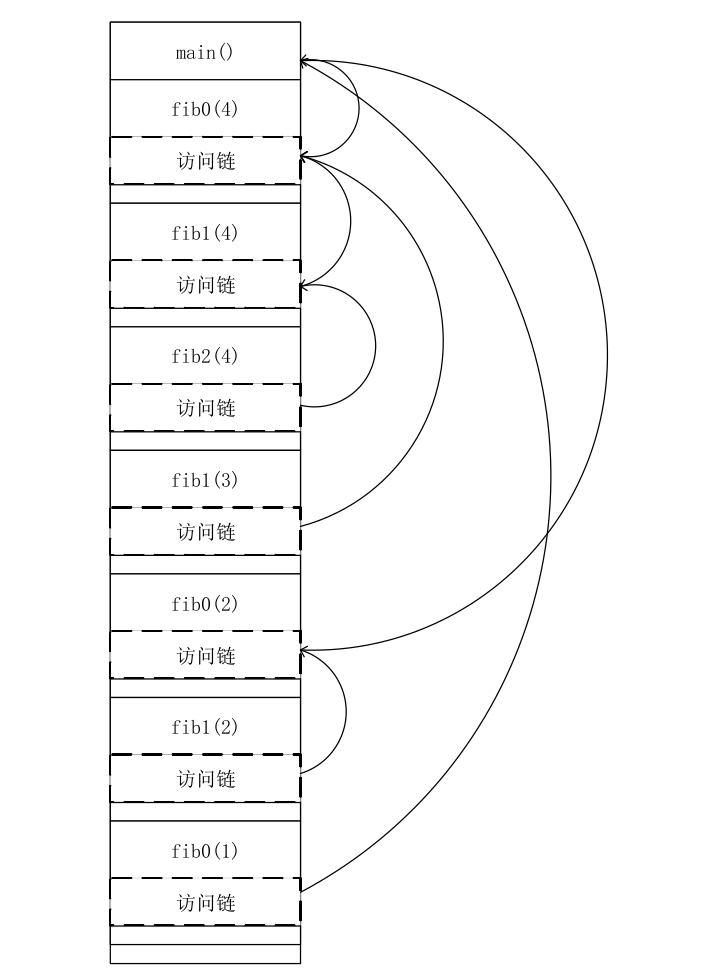
\includegraphics[scale = 0.4]{./fig/7-3-1.png}
\end{figure}

$7.3.2$解:$display$表和活动记录栈如下图所示:
\begin{figure}[H]
  \centering
  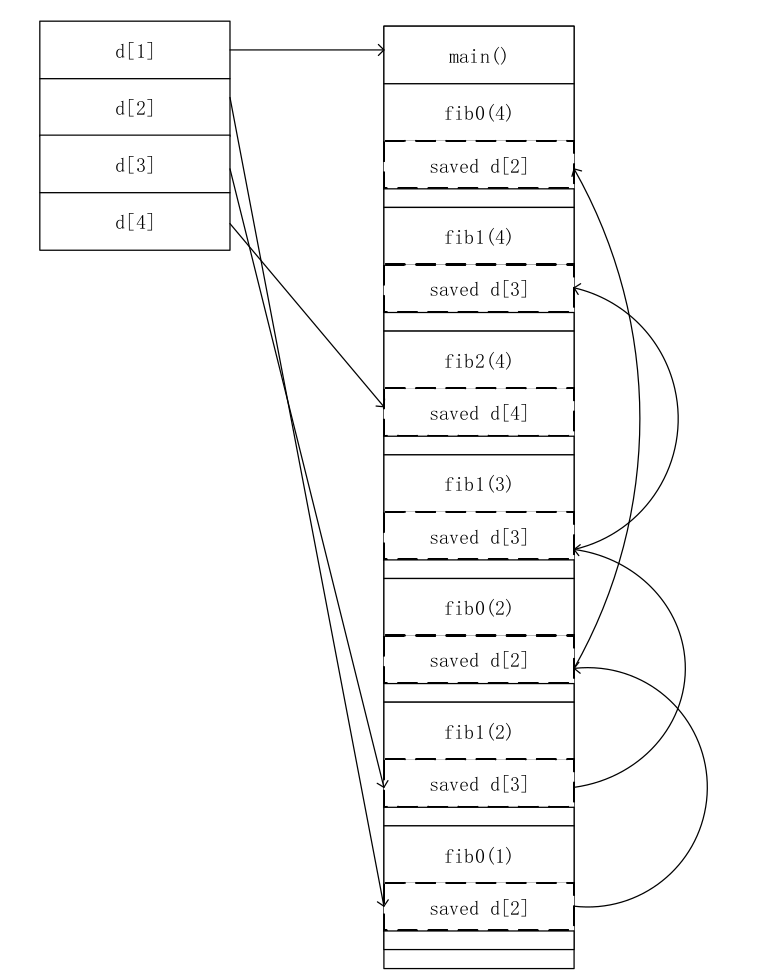
\includegraphics[scale = 0.4]{./fig/7-3-2.png}
\end{figure}
\end{document}


